% =====================================================================
%  BLOCCO 3 --- Radiazione di corpo nero e potenza assorbita
% =====================================================================

\section{Blocco 3 --- Sorgente a corpo nero}

% --- Slide: contesto fisico ---
\begin{frame}
\frametitle{Contesto fisico --- Plasma da fusione}

Il bolometro \`e impiegato per misurare la \textbg{radiazione totale}
emessa dal plasma in un tokamak.

\vspace{0.4em}
\begin{columns}[T]
  \begin{column}{0.55\textwidth}
    \textbf{Sorgente ipotizzata:}
    \begin{itemize}
      \item Corpo nero a temperatura del plasma di bordo
      \item $T_\text{source} = \SI{85}{\electronvolt}
            \approx \SI{9.9e5}{\kelvin}$
      \item Banda di frequenza: NIR $\to$ raggi~X
        \[
          f \in [3\times10^{14},\; 3\times10^{18}]\;\si{\hertz}
        \]
      \item Lunghezze d'onda: $\lambda \in [\SI{0.1}{\nano\meter},\; \SI{1000}{\nano\meter}]$
    \end{itemize}
  \end{column}
  \begin{column}{0.42\textwidth}
    \textbf{Obiettivo del Blocco 3:}
    \begin{enumerate}
      \item Calcolare la radianza spettrale $B(f,T)$
      \item Pesare con l'assorbanza del sensore $A(f)$
      \item Integrare su tutte le frequenze:\\
            $P_\text{abs} = \int B\,A\,\mathrm{d}f$
      \item Calcolare il rapporto\\
            $\eta = P_\text{abs} / P_\text{emit}$
      \item Studiare $\eta(T)$ al variare di $T$
    \end{enumerate}
  \end{column}
\end{columns}

\end{frame}

% --- Slide: formula di Planck ---
\begin{frame}
\frametitle{Radianza spettrale di Planck}

La \textbg{radianza spettrale} di un corpo nero a temperatura $T$ \`e:

\[
  B(f, T) = \frac{2\,h\,f^3}{c^2}
             \cdot \frac{1}{\exp\!\left(\dfrac{h\,f}{k_B\,T}\right) - 1}
  \quad \left[\si{\watt\per\meter\squared\per\steradian\per\hertz}\right]
\]

\vspace{0.3em}
\begin{columns}[T]
  \begin{column}{0.48\textwidth}
    \textbf{Costanti fisiche:}
    \begin{itemize}
      \item $h = \SI{6.626e-34}{\joule\second}$
      \item $c = \SI{3e8}{\meter\per\second}$
      \item $k_B = \SI{1.381e-23}{\joule\per\kelvin}$
    \end{itemize}
  \end{column}
  \begin{column}{0.48\textwidth}
    \textbf{Implementazione MATLAB:}
    \begin{itemize}
      \item 500 punti in \texttt{logspace} su $[3\times10^{14}, 3\times10^{18}]$\,Hz
      \item Integrazione numerica con la regola dei trapezi:
        \[
          P_\text{abs} = \int B(f,T)\,A(f)\,\mathrm{d}f
                       \approx \sum_i \Delta f_i\,B_i\,A_i
        \]
    \end{itemize}
  \end{column}
\end{columns}

\end{frame}

% --- Slide: assorbanza del platino ---
\begin{frame}
\frametitle{Assorbanza spettrale del platino}

Il sensore in platino non assorbe uniformemente su tutta la banda.
L'\textbg{assorbanza} $A(f) \in [0,1]$ \`e modellata con 7 punti chiave
e interpolazione lineare in spazio log-log:

\vspace{0.3em}
\begin{center}
\begin{tabular}{lc}
  \toprule
  Frequenza $f$~[Hz] & $A(f)$ \\
  \midrule
  $3\times10^{14}$ (NIR)     & 0.20 \\
  $6\times10^{14}$ (Vis.)    & 0.30 \\
  $1.5\times10^{15}$ (UV)    & 0.50 \\
  $3\times10^{15}$ (UV vuoto)& 0.65 \\
  $3\times10^{16}$ (EUV)     & 0.80 \\
  $3\times10^{17}$ (Molli~X) & 0.95 \\
  $3\times10^{18}$ (Duri~X)  & 0.99 \\
  \bottomrule
\end{tabular}
\end{center}

\vspace{0.2em}
\small
Il platino \`e trasparente nell'IR e quasi opaco ai raggi~X, comportamento
tipico dei metalli a film sottile usati nei bolometri da fusione.

\end{frame}

% --- Slide: risultati Planck + assorbanza ---
\begin{frame}
\frametitle{Risultati --- Radianza, assorbanza e integrando}

\begin{center}
  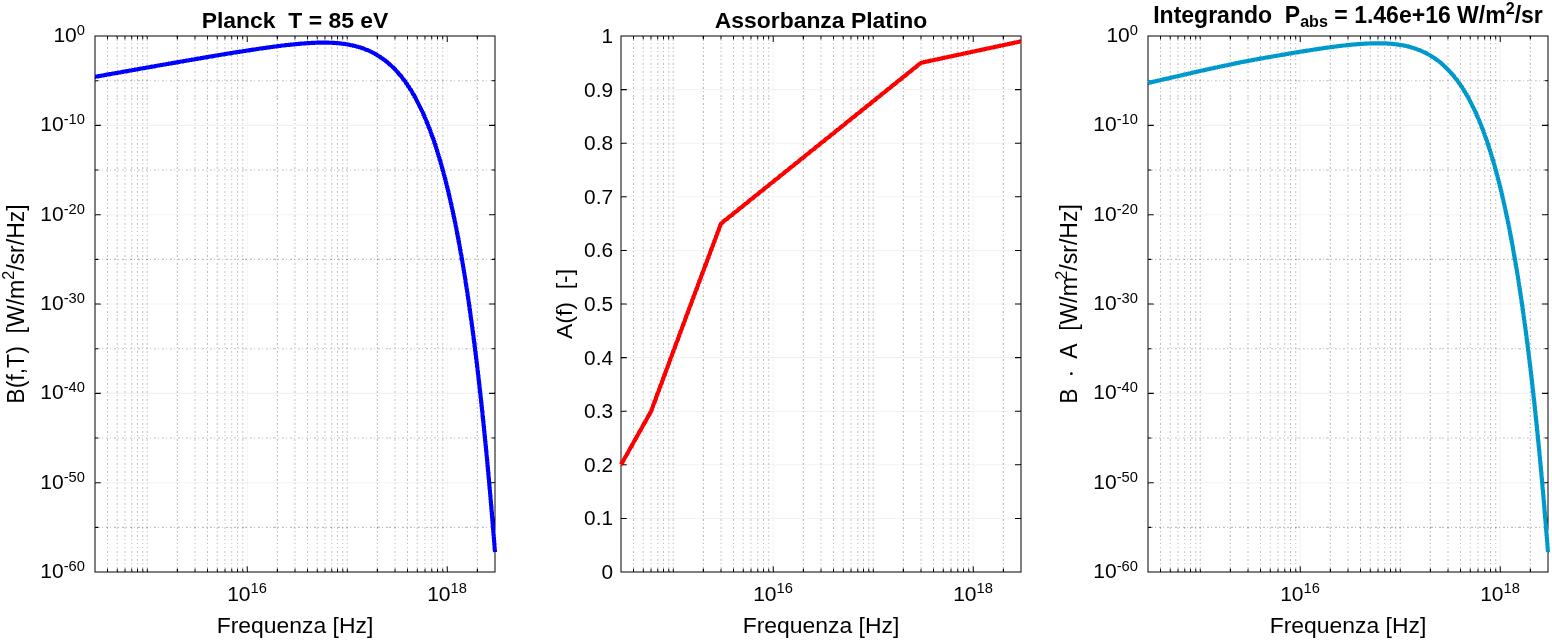
\includegraphics[width=0.92\textwidth]{blocco3_risultati.png}
\end{center}

\vspace{-0.3em}
\small
\textit{Sinistra}: $B(f,T)$ del corpo nero a $T = \SI{85}{\electronvolt}$.
\textit{Centro}: assorbanza $A(f)$ del platino.
\textit{Destra}: integrando $B(f)\cdot A(f)$ e potenza assorbita
$P_\text{abs} = \int B\,A\,\mathrm{d}f$.

\end{frame}

% --- Slide: potenza assorbita risultato numerico ---
\begin{frame}
\frametitle{Potenza assorbita --- risultato numerico}

A $T_\text{nom} = \SI{85}{\electronvolt}$, l'integrazione numerica d\`a:

\vspace{0.3em}
\begin{center}
\begin{tabular}{lrl}
  \toprule
  Grandezza & Valore & Unit\`a \\
  \midrule
  $P_\text{emit} = \int B\,\mathrm{d}f$ & dipende da $T$ & W/m$^2$/sr \\
  $P_\text{abs}  = \int B\cdot A\,\mathrm{d}f$ & $< P_\text{emit}$ & W/m$^2$/sr \\
  $\eta = P_\text{abs}/P_\text{emit}$ & vedi tabella & -- \\
  \bottomrule
\end{tabular}
\end{center}

\vspace{0.4em}
Variazione intorno a $T_\text{nom}$ con passo $\Delta T = \SI{10}{\electronvolt}$:

\vspace{0.2em}
\begin{center}
\small
\begin{tabular}{ccc}
  \toprule
  $T$~[eV] & $\eta = P_\text{abs}/P_\text{emit}$~[\%] & Nota \\
  \midrule
  55  & (minimo) & spettro spostato verso NIR \\
  \textbg{85}  & \textbg{(nominale)} & \textbg{punto di lavoro} \\
  115 & (massimo) & spettro spostato verso X \\
  \bottomrule
\end{tabular}
\end{center}

\vspace{0.3em}
\small
Il rapporto $\eta$ \textbg{cresce con $T$}: a temperature pi\`u elevate
lo spettro di Planck si sposta verso frequenze pi\`u alte, dove $A(f)$
del platino \`e maggiore (legge di Wien: $f_\text{max} \propto T$).

\end{frame}

% --- Slide: efficienza assorbimento vs T ---
\begin{frame}
\frametitle{Efficienza di assorbimento vs temperatura}

\begin{center}
  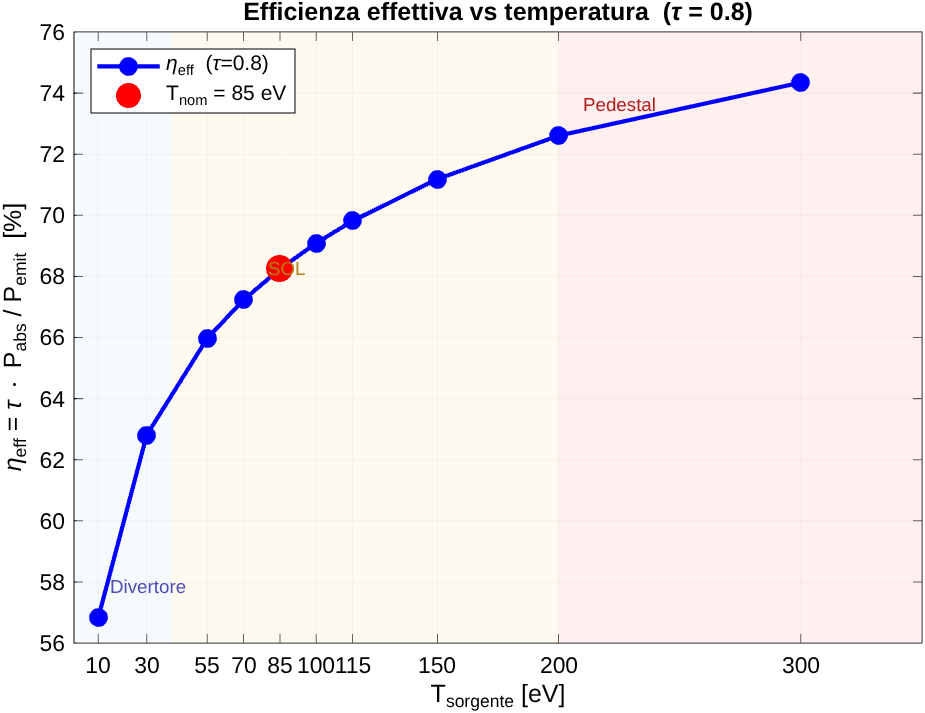
\includegraphics[width=0.72\textwidth]{blocco3_assorbimento.png}
\end{center}

\vspace{-0.3em}
\small
Il punto rosso indica $T_\text{nom} = \SI{85}{\eV}$.
La curva \`e monotona crescente: a temperature pi\`u alte il picco
dello spettro di Planck si sposta verso l'EUV/raggi~X dove il platino
assorbe di pi\`u. Il bolometro \`e quindi \textbg{pi\`u sensibile}
(a parit\`a di geometria) quando misura plasmi pi\`u caldi.

\end{frame}

% --- Slide: conclusioni ---
\begin{frame}
\frametitle{Conclusioni}

\begin{columns}[T]
  \begin{column}{0.55\textwidth}
    \textbf{Blocco 1 --- Modello diretto}
    \begin{itemize}
      \item Catena lineare $P \to \Delta T \to \Delta R \to \Delta V$
      \item Saturazione termica domina a $P_\text{sat} = \SI{5}{\milli\watt}$
    \end{itemize}

    \vspace{0.4em}
    \textbf{Blocco 2 --- Rumore}
    \begin{itemize}
      \item Rumore gaussiano $V_\text{noise} = \SI{10}{\micro\volt}$
      \item $\mathrm{NEP} \approx \SI{2.56}{\micro\watt}$
      \item Range dinamico $\approx 3$ decadi
    \end{itemize}
  \end{column}
  \begin{column}{0.42\textwidth}
    \textbf{Blocco 3 --- Corpo nero}
    \begin{itemize}
      \item Spettro di Planck a $T = \SI{85}{\electronvolt}$
      \item Assorbanza Pt da NIR a raggi~X
      \item $\eta = P_\text{abs}/P_\text{emit}$ cresce con $T$
      \item Il bolometro in Pt \`e pi\`u efficiente\\
            per plasmi pi\`u caldi
    \end{itemize}

    \vspace{0.4em}
    \begin{block}{Risultato chiave}
      La legge di Wien sposta il picco verso le X
      al crescere di $T$: il platino assorbe meglio
      l\`i, quindi $\eta(T)$ \`e crescente.
    \end{block}
  \end{column}
\end{columns}

\end{frame}
